
\begin{figure}[H]
  \centering
  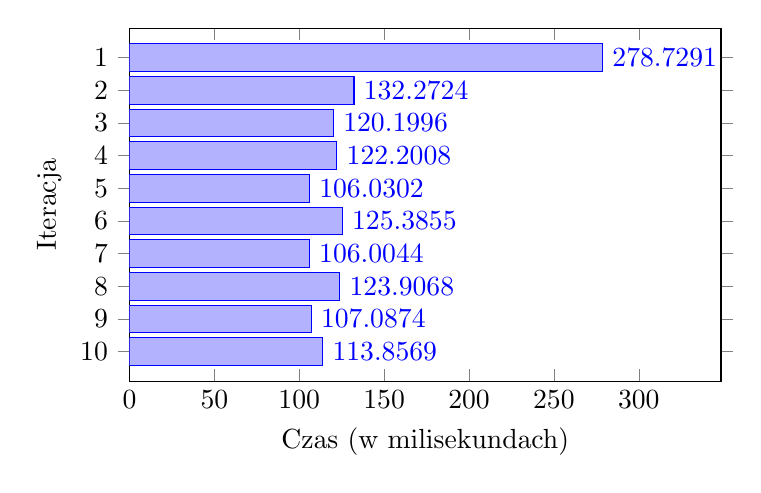
\begin{tikzpicture}
  
    \begin{axis} [
      xbar = .05cm,
      nodes near coords,
      nodes near coords style={
        /pgf/number format/precision=4,
      },
      xmin = 0,
      ytick = data,
      enlarge x limits = {value = .25, upper},
      symbolic y coords = {10,9,8,7,6,5,4,3,2,1},
      xlabel=Czas (w milisekundach),
      ylabel=Iteracja,
      width=0.75\textwidth,
      height=0.5\textwidth
    ]
    
      \addplot coordinates {(278.7291000187397,1) (132.27239999175072,2) (120.1996000111103,3) (122.20080000162125,4) (106.03020000457764,5) (125.38549998402596,6) (106.00440001487732,7) (123.90680000185966,8) (107.08740001916885,9) (113.85690000653267,10)};
      
    \end{axis}
  
  \end{tikzpicture}
  \caption{Wynik testów przykładu 1 [\ref{lst:wydajnosc-przyklad-p-1}]}
  \label{fig:wynik-przyklad-0}
\end{figure}
